\begin{pastexam}[label={px:ntu-106-im-it-01}]{臺大資管所 106 學年度 問答題第 1 題}
（問答；20 分）

When implementing the operations for a binary search tree, the notion of ``inorder successor''
(alternatively, inorder predecessor) is very useful.
\begin{enumerate}[label=(\alph*)]
\item Define the notion and explain why it is needed using examples.
\item Implement an algorithm in C, C++, or Java (choose one programming language) for finding the
inorder successor of a given node. The more efficient your implementation is, the more points you
will be credited.
\end{enumerate}
\end{pastexam}

\begin{pastsoln}
以下假設鍵值互不相同，用下面這棵二元搜尋樹當例子。

\begin{center}
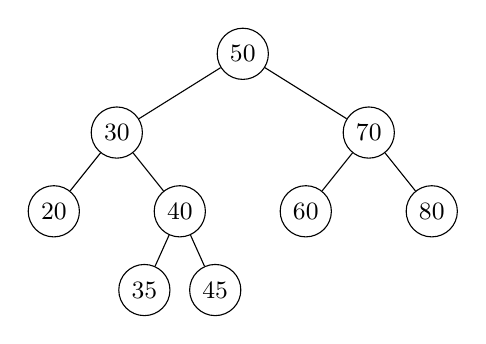
\begin{tikzpicture}[every node/.style={circle,draw,minimum size=6.5mm,inner sep=0pt,font=\small},
  level distance=10mm, level 1/.style={sibling distance=32mm}, level 2/.style={sibling distance=16mm},
  level 3/.style={sibling distance=9mm}]
\node {50}
  child {node {30} child {node {20}} child {node {40} child {node {35}} child {node {45}}}}
  child {node {70} child {node {60}} child {node {80}}};
\end{tikzpicture}
\end{center}
中序走訪的順序是 $20, 30, 35, 40, 45, 50, 60, 70, 80$。

\textbf{(a) 定義。} 節點 $x$ 的\textbf{中序後繼}（inorder successor）是中序走訪時緊接在 $x$
後面被拜訪的節點；中序走訪最後一個節點沒有後繼。 二元搜尋樹的中序就是鍵值由小到大的順序
（資結書定理~9.1），所以 $x$ 的後繼也就是「鍵值比 $x.\mathit{key}$ 大的節點中，鍵值最小的那
一個」。 中序前驅（predecessor）左右對調：鍵值比 $x.\mathit{key}$ 小的節點中最大的那一個。
上圖中 $30$ 的後繼是 $35$，$45$ 的後繼是 $50$，$80$ 沒有後繼。

找後繼分兩種情況（資結書第~9.1~節）：
\begin{itemize}
\item $x$ 有右子樹：後繼是右子樹的最小值，也就是從 $x.\mathit{right}$ 一路往左走到底。 例：
$30$ 的右子樹是 $\{35, 40, 45\}$，往左走到底是 $35$。
\item $x$ 沒有右子樹：往上找，第一個「$x$ 落在它左子樹裡」的祖先就是後繼。 例：$45$ 是 $40$
的右子節點，$40$ 是 $30$ 的右子節點，$30$ 是 $50$ 的左子節點，所以後繼是 $50$。 一路往上都是
從右邊上來、走到根還沒停（例如 $80$），就沒有後繼。
\end{itemize}

\textbf{為什麼需要它}，舉三個用途：
\begin{enumerate}
\item \textbf{刪除有兩個子節點的節點。} 直接拿掉會留下兩棵子樹，要找一個鍵值來頂替這個位置，
又不能破壞「左小右大」。 後繼正好合適：它比左子樹全部都大，又是右子樹裡最小的。 例如刪除
$30$：把 $35$ 搬到 $30$ 的位置，再刪掉原來的 $35$（它是右子樹的最小值，沒有左子節點，最多一
個子節點，好刪），得到根 $50$、左子節點 $35$（子節點 $20$、$40$，$40$ 只剩右子節點 $45$）。
這就是資結書虛擬碼~9.7 的做法，用前驅頂替也可以。
\item \textbf{依序走訪（迭代器）。} 從最小值開始一直取後繼，就能一個一個由小到大輸出，不必用
遞迴或堆疊。 範圍查詢「列出 $[33, 47]$ 之間的鍵值」：先找到第一個 $\ge 33$ 的節點 $35$，再
連取後繼 $40, 45$，碰到 $50 > 47$ 就停。
\item \textbf{回答「下一個」的查詢。} 例如鍵值是會員編號，問「編號 $45$ 之後的下一位是誰」，
答案就是 $45$ 的後繼 $50$。 引線二元樹（資結書第~7.5~節）也是把後繼直接存在空的右指標裡，
讓中序走訪更快。
\end{enumerate}

\textbf{(b) 實作。} 用 C。 節點存父指標 \texttt{parent}，照上面兩種情況寫（資結書虛擬碼~9.4）：

\begin{minted}[fontsize=\small]{c}
typedef struct Node {
    int key;
    struct Node *left, *right, *parent;
} Node;

Node *tree_minimum(Node *x)
{
    while (x->left != NULL)
        x = x->left;
    return x;
}

/* 回傳 x 的中序後繼；x 是最大值時回傳 NULL */
Node *inorder_successor(Node *x)
{
    if (x->right != NULL)            /* 情況一：右子樹的最小值 */
        return tree_minimum(x->right);
    Node *y = x->parent;             /* 情況二：往上找 */
    while (y != NULL && x == y->right) {
        x = y;
        y = y->parent;
    }
    return y;
}
\end{minted}

如果節點沒有父指標，就從根往下找（資結書虛擬碼~9.5）：沿著搜尋 $x.\mathit{key}$ 的路往下走，
每次往左轉時那個節點比 $x.\mathit{key}$ 大，是候選，越晚的候選越小，記住最後一個。

\begin{minted}[fontsize=\small]{c}
Node *successor_from_root(Node *root, int k)
{
    Node *s = NULL;                  /* 目前看到比 k 大的最小節點 */
    while (root != NULL) {
        if (k < root->key) {
            s = root;
            root = root->left;
        } else {
            root = root->right;
        }
    }
    return s;
}
\end{minted}

\textbf{正確性。} 有父指標的版本：
\begin{itemize}
\item 情況一：右子樹的鍵值都大於 $x.\mathit{key}$。 不在右子樹裡、又比 $x.\mathit{key}$ 大的
節點 $z$，一定是某個祖先 $a$（$x$ 在 $a$ 的左子樹裡）本身或 $a$ 的右子樹裡的節點，$z \ge a$，
而 $a$ 比它整棵左子樹都大，當然也比 $x$ 的右子樹大。 所以後繼是右子樹的最小值。
\item 情況二：$x$ 沒有右子樹。 迴圈每一步都是從右子節點走到父節點，所以迴圈結束時，原本的
$x$（記作 $x_0$）是目前 $x$ 這棵子樹裡最右邊、也就是最大的節點；而目前的 $x$ 是 $y$ 的左子
節點。 比 $x_0$ 大的節點都不在這棵子樹裡，其中 $y$ 比它的整棵右子樹小；更上面的祖先若比 $y$
小，就比整棵 $y$ 子樹都小（也小於 $x_0$），若比 $y$ 大，連同它們的右子樹都比 $y$ 大。 所以
$y$ 是比 $x_0$ 大的最小鍵值。 走到根還沒停（$y = \NIL$）表示 $x_0$ 是整棵樹最右邊的節點，
沒有後繼。
\end{itemize}
從根往下的版本：比 $k$ 大的節點裡最小的那一個一定在搜尋路徑上
（否則它和 $k$ 之間會隔著路徑上的某個節點），而路徑上比 $k$ 大的節點正是往左轉的那些，它們
沿路越來越小，最後一個就是答案。

\textbf{複雜度。} 兩個版本都只沿一條根到葉的路徑走一次（情況一往下、情況二往上），時間
$O(h)$，$h$ 是樹高，額外空間 $O(1)$。 樹是平衡的（AVL、紅黑樹）時 $h = O(\log n)$；退化成
一條鏈時最壞 $O(n)$。 相比之下，先做一次完整的中序走訪再找 $x$ 的下一個要 $\Theta(n)$ 時間，
所以上面的寫法比較有效率。 另外，從最小值開始連續取 $n - 1$ 次後繼，總共只花 $O(n)$：每條邊
最多往下走一次、往上走一次。
\end{pastsoln}
